% Options for packages loaded elsewhere
\PassOptionsToPackage{unicode}{hyperref}
\PassOptionsToPackage{hyphens}{url}
%
\documentclass[
]{article}
\usepackage{amsmath,amssymb}
\usepackage{lmodern}
\usepackage{iftex}
\ifPDFTeX
  \usepackage[T1]{fontenc}
  \usepackage[utf8]{inputenc}
  \usepackage{textcomp} % provide euro and other symbols
\else % if luatex or xetex
  \usepackage{unicode-math}
  \defaultfontfeatures{Scale=MatchLowercase}
  \defaultfontfeatures[\rmfamily]{Ligatures=TeX,Scale=1}
\fi
% Use upquote if available, for straight quotes in verbatim environments
\IfFileExists{upquote.sty}{\usepackage{upquote}}{}
\IfFileExists{microtype.sty}{% use microtype if available
  \usepackage[]{microtype}
  \UseMicrotypeSet[protrusion]{basicmath} % disable protrusion for tt fonts
}{}
\makeatletter
\@ifundefined{KOMAClassName}{% if non-KOMA class
  \IfFileExists{parskip.sty}{%
    \usepackage{parskip}
  }{% else
    \setlength{\parindent}{0pt}
    \setlength{\parskip}{6pt plus 2pt minus 1pt}}
}{% if KOMA class
  \KOMAoptions{parskip=half}}
\makeatother
\usepackage{xcolor}
\usepackage[margin=1in]{geometry}
\usepackage{graphicx}
\makeatletter
\def\maxwidth{\ifdim\Gin@nat@width>\linewidth\linewidth\else\Gin@nat@width\fi}
\def\maxheight{\ifdim\Gin@nat@height>\textheight\textheight\else\Gin@nat@height\fi}
\makeatother
% Scale images if necessary, so that they will not overflow the page
% margins by default, and it is still possible to overwrite the defaults
% using explicit options in \includegraphics[width, height, ...]{}
\setkeys{Gin}{width=\maxwidth,height=\maxheight,keepaspectratio}
% Set default figure placement to htbp
\makeatletter
\def\fps@figure{htbp}
\makeatother
\setlength{\emergencystretch}{3em} % prevent overfull lines
\providecommand{\tightlist}{%
  \setlength{\itemsep}{0pt}\setlength{\parskip}{0pt}}
\setcounter{secnumdepth}{5}
\usepackage{amsmath}
\usepackage{amssymb}
\usepackage{float}
\usepackage{titling}
\usepackage[citestyle=authoryear, backend=biber, style=apa]{biblatex}
\bibliography{references}
\usepackage{xcolor}
\ifLuaTeX
  \usepackage{selnolig}  % disable illegal ligatures
\fi
\IfFileExists{bookmark.sty}{\usepackage{bookmark}}{\usepackage{hyperref}}
\IfFileExists{xurl.sty}{\usepackage{xurl}}{} % add URL line breaks if available
\urlstyle{same} % disable monospaced font for URLs
\hypersetup{
  pdfauthor={Group II},
  hidelinks,
  pdfcreator={LaTeX via pandoc}}

\DeclareLanguageMapping{english}{english-apa}
\addbibresource{literature.bib}

\title{The Price Air Pollution\\
1436 - Spatial Economics}
\author{Group II}
\date{12/31/2022}

\begin{document}
\maketitle

\begin{center}
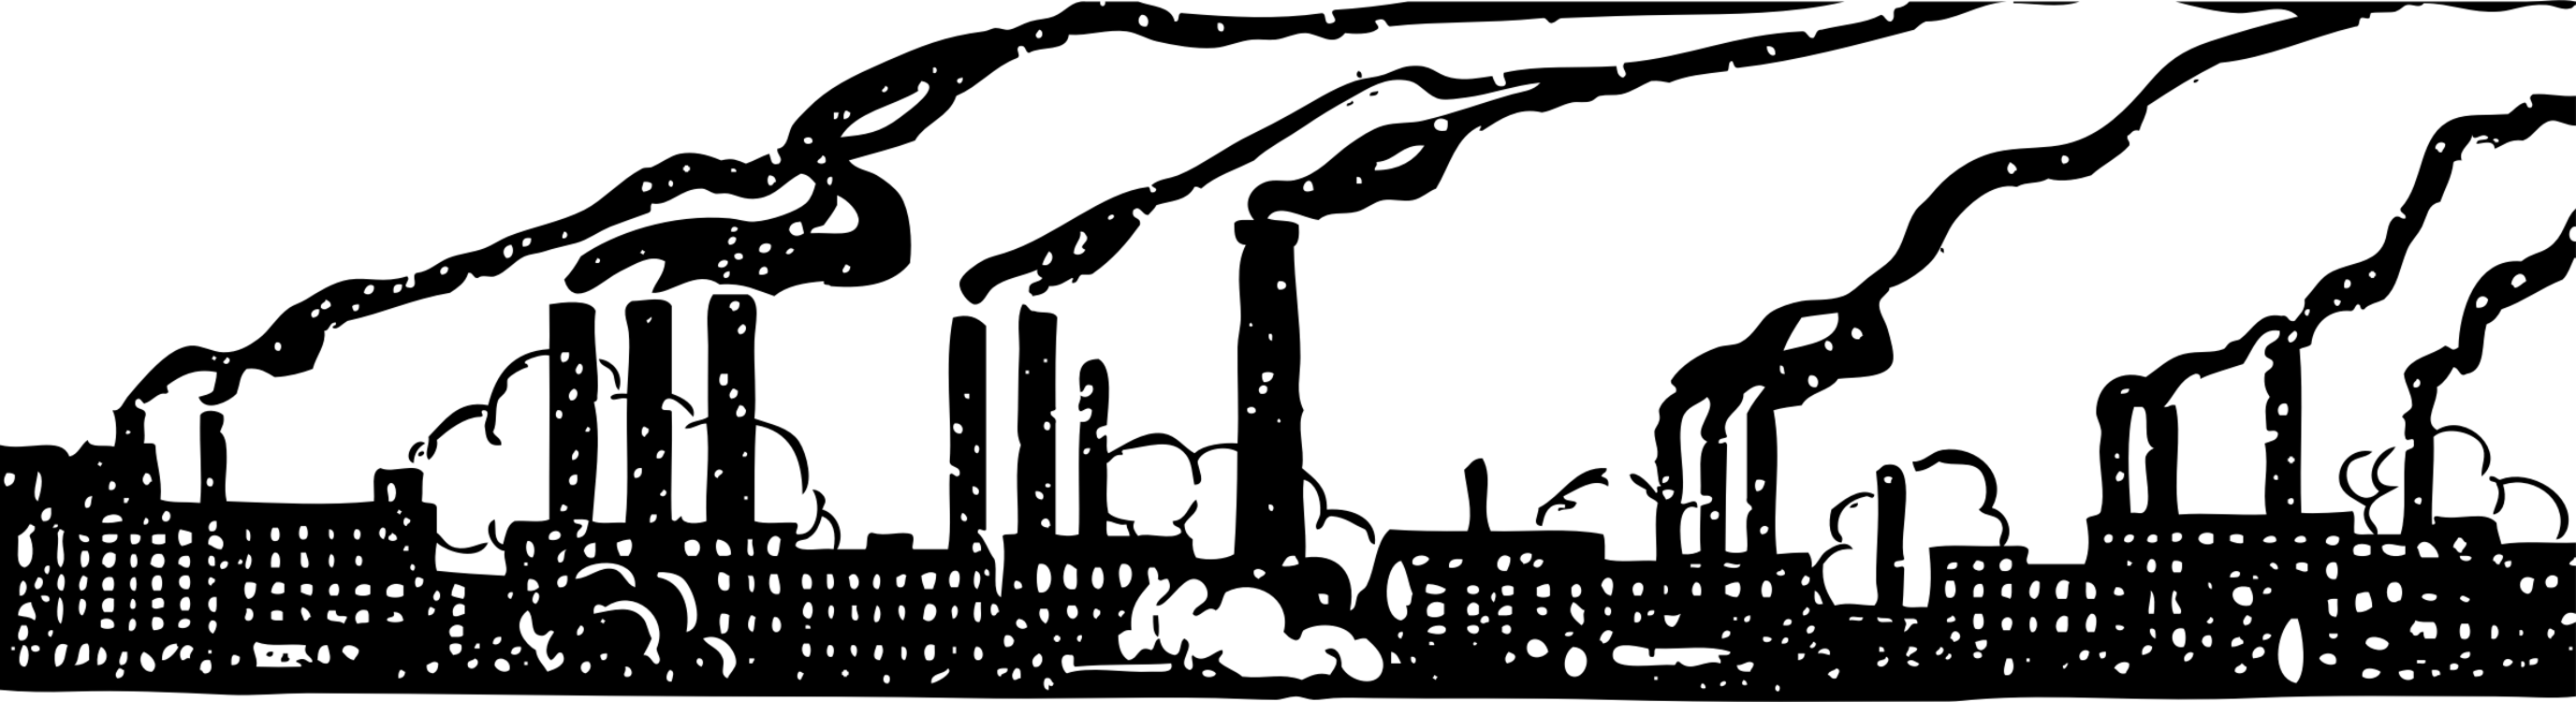
\includegraphics[width = 380pt]{pollution.png} 
\end{center}
\thispagestyle{empty}
\begin{abstract}
	
\end{abstract}
\newpage
\pagenumbering{arabic}

\hypertarget{introduction}{%
\section{Introduction}\label{introduction}}
Air pollution in China is a persistent issue, but how serious is it? 
In 2019 the major premature death causes in China were cardiovascular diseases totaling 43 percent, followed by malignant neoplasms (26 percent), respiratory diseases (10 percent), unintentional injuries (6 percent) and neurological conditions (4 percent). Other conditions that accounted for between 3 and 1 percent of premature deaths, in descending order, were digestive diseases, genitourinary diseases, respiratory infections, diabetes mellitus and infectious and parasitic diseases. %https://www.who.int/data/gho/data/themes/mortality-and-global-health-estimates/ghe-leading-causes-of-death
Due to the outdated benefit structure in China, which will be discussed in more detail in chapter xyz, it is mainly the inhabitants of rural areas who benefit the least. 

Thus air pollution has its consequences and these are reflected in the health of the population which accordingly leads to an increase in health care  expenditures. 







\hypertarget{literature review}{%
\section{Literature review}\label{Literature review}}

\subsection{Effects of air pollution on health}

Analysing the effect of air pollution on health expenditures implicitly implies the aforementioned causal transition dependencies. Various studies have identified direct effects of exposure to air pollution on health. %(Quellen einfügen bei "various studies")

Franklin, Brook, Pope III (2015) and Fiordelisi et al. (2017) demonstrate that the risk of cardiovascular diseases and the triggering of acute cardiac events is increased by PM air pollution. The pathways through which this occurs include the generation of proinflammatory or oxidative stress mediators in the lung that enter the systemic circulation, the direct infiltration of certain particles or components into the cardiovascular tissue, or an imbalance of the autonomous nervous system. In that context, Hoek et. al (2013) quantify the effect of PM2,5 long-term exposure by conducting a meta-analytic review of previous studies. Their pooled estimate indicates an increase in all-cause mortality and cardiovascular mortality of 6 percent and 11 percent, respectively, if increments of PM2,5 are increased by 10-myg/m3. Equivalently, an increase in NO concentration of the same magnitude leads to an increased all-cause mortality of five percent. %https://www.sciencedirect.com/science/article/pii/S0146280615000043; https://ehjournal.biomedcentral.com/articles/10.1186/1476-069X-12-43; https://pubmed.ncbi.nlm.nih.gov/28303426/

tbd Respiratory diseases %https://www.ncbi.nlm.nih.gov/pmc/articles/PMC6033955/
tbd lung cancer %https://www.jstor.org/stable/3703988

tbd DALY %https://www.nature.com/articles/nature15371; https://www.sciencedirect.com/science/article/pii/S0140673616315975?ref=cra_js_challenge&fr=RR-1

Additionally, Zhao et al. suggest that based on recent findings air pollution may be involved in the development of autoimmune diseases such as diabetes mellitus, multiple sclerosis, or rheumatoid arthritis. The authors argue that air pollution can cause imbalances in T cells, the production of proinflammatory cytokines, oxidative stress, local pulmonary inflammation and methylation changes. These effects are involved with initiating or aggravating autoimmune diseases. %https://www.sciencedirect.com/science/article/pii/S1568997219300886



\subsection{Air pollutions policies from 2011 to 2018}

Air pollution in China has been a major public health problem for many years. However in recent years the government has taken various measures to address the issue. One of the main focuses of these measures has been to reduce emissions of particulate matter, sulfur dioxide and nitrogen oxides. 
In 2013, prompted by a period of heavy smog in eastern China, the government introduced an "Air Pollution Control Action Plan" to combat air pollution, which included specific targets for reducing particulate matter, sulfur dioxide, and nitrogen oxide emissions. More specifically, targets included, among others, reducing PM10 concentrations in cities by more than 10 percent and reducing PM2.5 concentrations in the Beijing-Tianjin-Hebei, Yangtze River Delta and Pearl River Delta regions of around 25, 20 and 15 percent, respectively. %Quellen: https://english.mee.gov.cn/News_service/infocus/201309/t20130924_260707.shtml; https://www.mdpi.com/1660-4601/13/12/1219

Furthermore, the 13th Five-Year Plan (2016-2020) also set a target to reduce PM2.5 concentrations in areas heavily affected by air pollution by 18 percent by 2020. Targets have also been set for reducing sulfur dioxide and nitrogen oxide emissions by 15 percent and 15 percent, respectively, compared to 2015 levels. %Quelle: https://en.ndrc.gov.cn/policies/202105/P020210527785800103339.pdf
Huang, Pan, Guo, Li (2018) indicate in their analysis, in which they map the national air quality in 74 cities that the issued Air Pollution Prevention and Control Action Plan (APPCAP) in 2013 has shown effect. Between 2013 and 2017 PM2.5 concentrations have reduced in average by about 33 percent, and PM10 concentrations by about 28 percent. Sulfur dioxide concentrations have reduced as well with an average reduction of about 54 percent. Nitrogen Oxides emissions, however, have not significantly decreased. %Quelle: https://www.sciencedirect.com/science/article/pii/S2542519618301414?ref=cra_js_challenge&fr=RR-1

In summary, a number of measures have been taken by the Chinese government from 2011 to 2018 to reduce air pollution, including stricter emission standards for vehicles, power plants and industrial facilities, and the closure or upgrading of older, heavily polluting factories, which were partially effective. %https://www.mdpi.com/1660-4601/13/12/1219 

\subsection{Organization of the Chinese Healthcare System}
This chapter will provide an overview of the structure of the Chinese Health Care System and highlight one of its main characteristics: It creates inequalities between the urban and rural population. 

In the late 1990s, the years of the opening and globalization as \textcite{kanbur_fifty_2005} describes it, China developed from a centralized to an open market economy, there have been several reforms in the country, including in the health care system. 

According to \textcite{hougaard_chinese_2011} no longer the central Chinese government but rather the different Provinces are responsible for the financing and administrating the health care system, instead of a . This, since funding is provided through taxation, in turn led to strong inequalities between the rich coastal regions and the impoverished rural regions in the east of the country. The Chinese health care system is characterized by the division of the population between two groups: The proportion of the population living in the urban and rural areas. 

Before we delve deeper into the structure and allocation of the Chinese health care system, it is worth mentioning how social benefits are allocated in China. \cite{liu_institution_2005} describes The Hukou (eng. "individual origin" or also Huji eng. "household origin") is the government's official residence registration. This was introduced in the 1950s with the aim of. 

"...to maintain social order, protect the rights and interests of citizens, and serve the construction of socialism."

Because rural areas can further absorb and make use of surplus labor, the central government thought that the majority of the population should live there.
Domestic migration of people was also viewed as dangerous because it could result in city overpopulation and endanger farm production.
Domestic migration was likewise discouraged by the federal government.
The central government closely regulated migration flows, and only recently have these limitations been loosened, in the era of Mao Zhedong. This doesn't imply that the hukou system is no longer in place; rather, it only means that, for instance, rural dwellers can move to a city but won't be eligible for any social benefits there and will have to make due with their own resources.

\section{Data} \label{Data}

\section{Methodology}
%Use of panel data models
As already discussed in section \ref{Literature review}, the possibility of a spatial autoregressive process (SAR) is rather unlikely considering the Hukou system. We therefore excluded the possibility of a SAR component before using statistical testing to determine the final model.\\
We started the testing procedure by using the (Spatial) Hausmann Test to decide whether fixed or random effects suit the data better. The test strongly indicated the usage of a fixed effects model over time, which is in line with the intuition as China's provinces are heterogenerous and eliminating time constant features such as geographic differences seems like a reasonable approach.\\
In the following a Lagrange Mulitplier Test to decide whether a spatial error model (SEM) should be used. We could not reject the $H_0$ of a OLS model. Therefore, we continued to use a spatial lag in X (SLX) model, whose lag components can directly be tested by t-tests. The inclusion of a SLX component comes from the fact that air pollution of one province is likely to influence air pollution of neighbouring provinces. But, as already discussed in section \ref{Data}, it is not known whether the emission variables are only total emmission in a provinces that were also created in this province or if some smoothing of the data was already applied such that some distance travelled by means of kernel distribution or similar is used in order to account the effect on neighbouring provinces. The introduction of spatial lags concerning the air pollution will not cause any harm other than potential multicolinearity issues if they are in fact redundant.\\
The next step was to check to possible presence of heteroscedastic and serial correlated errors. Firstly, a Breusch-Pagan test was used to test for heteroscedasticity. Here we could reject the Null-Hypothesis of homoscedastic errors. Secondly, a Durbin-Watson test was conducted to test for serial correlation. The test strongly suggested serial correlation. As a result, we used a robust variance covariance matrix in order to account for this error structure and improve the reliability of our results\\
For the identification of the model, a general-to-specific approach was utilized, where we started with all reasonable variables and potential lags and eliminated them iteratively with the use of t-tests.\\
As a robustness check of our results, we used a feasible generalized least square model. Very similar to the SLX model we use a robust variance covavariance matrix that is corrected for heteroscedasticity and serial correlation. Also, the most general model is assumed again and variables are eliminated one-by-one.\par
Some variables of interest are in monetary terms. To account for the mere growth in these variables due to increased prices we adjust every monetary variables (X) by the general consumer price index (CPI)
$$\widetilde{X} = \frac{X}{CPI/100}.$$
The CPI is divided by 100 as it is reported with baseline value 100.\\
Additionally, on every variable a logarithmic transformation was used. The reason for this is twofold. To begin with it might further help with the heteroscedastic and serially correlated errors and therefore provide more reliant estimates. And it also helps to make the interpretation of the estimates more intuitively. One exception to this procedure is the share of working population, as this variables already presents a share of the whole population, a further transformation would make its interpretation meaningless.\\



\section{Results}
As previously outlined, the models presented in the table below were obtained using the general to specific model selection procedure. Starting from the model with all controls, statistically insignificant explanatory control variables were subsequently removed one at a time. During this process, the sign as well as the significance of our pollution variables were very sensitive to small changes in the model, i.e., we observed large changes in obtained estimates over a single iteration of the general to specific selection procedure. Accordingly, the presented results are to be interpreted cautiously. The unstable coefficient estimates are most likely caused by a combination of highly collinear explanatory variables and the absence of important variables that drive health care expenditures in our model.\\ Nevertheless, some key takeaways can be made. We observe that in our model, which does not contain spatially lagged variables, that Particulate Matter Emissions have a significant effect while in the SLX model this is not the case. This might be due to the mentioned multicollinearity problems, as all pollution variables exhibit a positive spatial correlation. The negative and significant effect of Sulphur Gas emissions, is most likely also a result of the multicolliniearity in our model. Especially, given that the spatial lag features a positive and significant coefficient, there is no sensible interpretation to be made. The key takeaway should thus be, even though we find a positive and significant effect of Particulate Matter Emission (fGLS) on Health Care Expenditure, the result is both unstable over iterations in our model selection procedure and also across model types. Further, given our modelling and identification strategy, we may not claim that the results represent a causal relationship between the examined variables.
\begin{table}[!htbp] \centering 
	\caption{Results fGLS \& SLX} 
	\label{} 
	\begin{tabular}{@{\extracolsep{5pt}}lcc} 
		\\[-1.8ex]\hline 
		\hline \\[-1.8ex] 
		& \multicolumn{2}{c}{\textit{Dependent variable:}} \\ 
		\cline{2-3} 
		\\[-1.8ex] & \multicolumn{2}{c}{ } \\ 
		\\[-1.8ex] & fGLS & SLX\\ 
		\hline \\[-1.8ex] 
		log(Disposable Income per Capita Rural) & 1.072$^{***}$ &  \\ 
		& (0.067) &  \\ 
		& & \\ 
		log(Disposable Income per Capita Urban) &  & 1.180$^{***}$ \\ 
		&  & (0.081) \\ 
		& & \\ 
		log(Forest Coverage Rate) & 0.490$^{***}$ & 0.287$^{**}$ \\ 
		& (0.102) & (0.144) \\ 
		& & \\ 
		log(Urban Population) & 0.308$^{**}$ & 0.504$^{***}$ \\ 
		& (0.145) & (0.135) \\ 
		& & \\ 
		log(Waste Gas Emissions Nitrogen) & $-$0.045 & 0.006 \\ 
		& (0.035) & (0.041) \\ 
		& & \\ 
		log(Waste Gas Emissions Particulate Matter) & 0.063$^{***}$ & 0.032 \\ 
		& (0.024) & (0.023) \\ 
		& & \\ 
		log(Waste Gas Emissions Sulphur) & $-$0.007 & $-$0.063$^{**}$ \\ 
		& (0.016) & (0.028) \\ 
		& & \\ 
		log(Waste Gas Emissions Nitrogen Lag) &  & $-$0.111 \\ 
		&  & (0.088) \\ 
		& & \\ 
		log(Waste Gas Emissions Particulate Matter Lag) &  & 0.117$^{***}$ \\ 
		&  & (0.040) \\ 
		& & \\ 
		log(Waste Gas Emissions Sulphur Lag) &  & 0.093$^{**}$ \\ 
		&  & (0.041) \\ 
		& & \\ 
		\hline \\[-1.8ex] 
		\hline 
		\hline \\[-1.8ex] 
		\textit{Note:}  & \multicolumn{2}{r}{$^{*}$p$<$0.1; $^{**}$p$<$0.05; $^{***}$p$<$0.01} \\ 
	\end{tabular} 
\end{table} 

\section{Conclusion}

\end{document}






